\section{Szerkesztő}
\rhead{Szerkesztő}

\subsection{Technológiák}

A 3D szerkesztő elkészítése számos technikai és tervezési problémát vetett fel. Egy olyan szoftver
megalkotása volt a cél, amely elég egyszerű ahhoz, hogy bárki használhassa, viszont megfelelően
eszközdús ahhoz, hogy képes legyen bonyolult épületek tervezésére is. Ezen feltételek
megfogalmazása után arra jutottunk, hogy a 3D szerkesztőt egy web alapú alkalmazás keretein belül
fogjuk megvalósítani.

Egy ilyen szoftver esetében nagyon fontos a sebesség, ezért úgy döntöttünk, hogy a
böngészőkben használt JavaScript helyett a sokkal gyorsabb --- ámbár fiatalabb és éretlenebb ---
WebAssembly\footnote{https://webassembly.org} technológiát fogjuk használni. Mivel a WebAssembly
önmagában csak egy utasításkészlet, szükségünk volt egy programozási nyelvre, amit lehetséges
WebAssembly utasításokra fordítani. Erre a célra a Rust\footnote{https://www.rust-lang.org}
programozási nyelvet választottuk. Ennek a döntésnek több oka is van:

\begin{itemize}
      \item Gyorsaság: A Rust egy rendszerközeli nyelv, hasonlóan a C-hez vagy C++-hoz, így rengeteg
            olyan optimalizáció valósítható meg, ami magasabb szintű nyelvekben nem lehetséges.

      \item Fejlett WebAssembly eszközök: Annak ellenére, hogy a nyelv viszonylag fiatal, rengeteg
            kiváló eszköz és könyvtár áll rendelkezésre a WebAssembly programok fejlesztésének
            elősegítéséhez. Ezek közül talán a legfontosabb a
            wasm-bindgen\footnote{https://github.com/rustwasm/wasm-bindgen} könyvtár, amellyel
            triviális feladattá válik a böngésző által használt JavaScript kód és a WebAssemblyre
            átforduló Rust kód összekötése.

      \item Tapasztalat: A fejlesztői csapat két tagja már használta a Rust programozási nyelvet a
            múltban, így elkerülhettük az új technológiák tanulásával járó problémákat.
\end{itemize}

\subsection{Működési elvek}

A használt technológiák kiválasztása után megkezdődött a szerkesztő működési elveinek felállítása.
Hamar eldöntöttük, hogy nagyrészt két, már létező szoftver eszközeiből szeretnénk ötleteket
meríteni.

Az egyik szoftver, a Blender\footnote{https://www.blender.org} egy általános rendeltetésű
háromdimenziós modellező program. Rendkívül sokoldalú és bonyolult, ezért csak néhány mechanizmust
ültettünk át a saját szerkesztőnkbe, például a kijelölés és a mozgatás módját.

\begin{figure}[h]
      \centering
      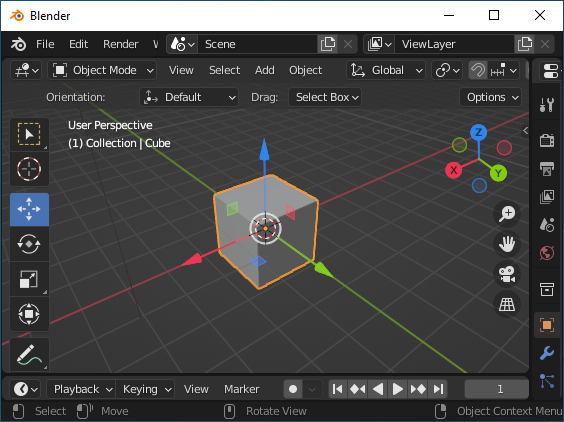
\includegraphics[width=0.5\textwidth]{parts/developer-documentation/editor/images/blender.png}
      \caption{Blender}
\end{figure}

A másik kiindulási pontként használt szoftver a
Valve Hammer Editor\footnote{https://developer.valvesoftware.com/wiki/Valve\_Hammer\_Editor}. A
program a Valve Software által fejlesztett Source játékmotor pályaszerkesztő alkalmazása. A Hammer
Editor egyik erőssége, és egyben az a tulajdonsága, amit mi is megvalósítottunk az, hogy benne
bármilyen komplex beltéri vagy kültéri jelenet lemodellezhető kisebb, egyszerűb alakzatok
felhasználásával.

\begin{figure}[h]
      \centering
      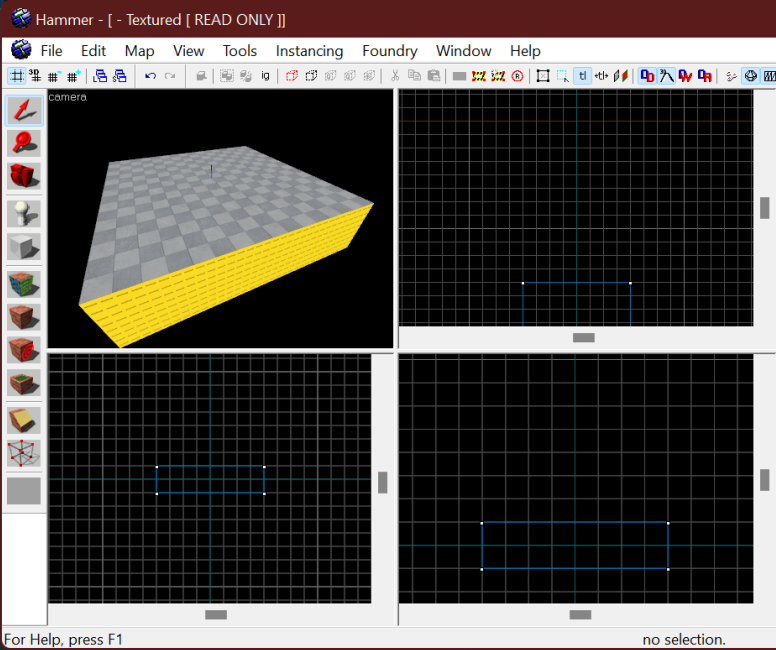
\includegraphics[width=0.5\textwidth]{parts/developer-documentation/editor/images/hammer.png}
      \caption{Valve Hammer Editor}
\end{figure}


\subsection{Kommunikáció a böngészővel}

Problémák és kihívások nem csak a tervezési fázisban bukkantak fel. Az egyik legelső probléma,
amivel fejlesztés közben találkoztunk, az a böngészővel való kommunikáció kérdése. Mivel a
JavaScript alapú felhasználói felület, és a Rust alapú szerkesztő valójában két független
alkalmazás, ezért ki kellett találni egy módszert az információmegosztásra. Az egyszerű
függvényhívások két okból nem feleltek meg. Először is, a JavaScript és WebAssembly kód natívan
csak egész számok átadására képes, ami mi céljainkhoz kevés. Másodszor, mivel a szerkesztő teljes
mértékben WebAssembly memóriában él, nincs semmilyen JavaScript objektum, aminek a függvényeit le
lehetne hívni.

Az első problémánkra a wasm-bindgen nevű Rust könyvtár adott megoldást. A wasm-bindgen lehetségessé
teszi az egész számoknál komplexebb adatstruktúrák átültétését Rust kódból JavaScript kódba, és
fordítva. A második probléma megoldása kicsit nehezebbnek bizonyult. Végül egy olyan
modellt valósítottunk meg, amiben a két fél két különböző módszert használ a kommunikációhoz.
Amikor a böngésző kommunikál a szerkesztővel, azt üzenetekkel teszi. Ezek az üzenetek egyszerű
adatstruktúrák amik egy aszinkron csatornán keresztül jutnak el a szerkesztőhöz. Amikor az
információátadás fordítva történik, a helyzet egyszerűbb: a JavaScript oldal egyszerűen átad egy
anoním függvényt a Rust oldalnak, amit aztán a szerkesztő szükség esetén meghív.

\subsection{3D grafika}

A szerkesztő egyik legfontosabb feladata, hogy képes legyen kirajzolni a jelenetet a képernyőre.
Ezt teszik lehetővé a különböző grafikus API-k, mint például az
OpenGL\footnote{https://www.opengl.org}, Vulkan\footnote{https://www.vulkan.org},
vagy böngésző esetén a WebGL\footnote{https://www.khronos.org/webgl}.
A Rust programozási nyelvhez rengeteg olyan könyvtár érhető el, ami ezeket az API-okat elérhetővé
teszi. Mi úgy döntöttünk, hogy a wgpu\footnote{https://github.com/gfx-rs/wgpu} könyvtárat fogjuk
használni. Ennek legfőbb oka az, hogy egy letisztult, biztonságos réteget húz a régies WebGL
interfészre.

\pagebreak

\subsection{Művelet alapú szerkesztés}

Az előzetes tervezési fázisban számunkra fontos kikötés volt, hogy a szerkesztés közben
megvalósulhasson az ún. non-destruktív munkamenet. Ez azt jelenti, hogy bármit, amit a felhasználó
megtesz, azt vissza lehet vonni. Ahhoz, hogy ez lehetséges legyen, valamilyen formában el kell
tárolni a múltbeli szerkesztési lépéseket. Végül úgy döntöttünk, hogy az egész szerkesztőt ezen
alapelv köré építjük fel. Létrehoztunk egy speciális adatszerkezetet, amely az összes elvégezhető
szerkesztési lépést képes eltárolni. Amikor a felhasználó változtat valamit a jeleneten, egy
ilyen adatstruktúra (művelet) kerül átadásra. Az végrehajtás után a szerkesztő felépíti az művelet
ellentétét, az inverz műveletet. Végül az inverz művelet eltárolásra kerül egy ún. visszavonási
veremben. Amikor a felhasználó kiadja a visszavonási parancsot, a visszavonási verem tetején lévő
művelet (ha létezik) újra végrehajtásra kerül, és belekerül egy másodlagos verembe, ami a visszavont
műveletek inverzeit tárolja. Ez azért szükséges, mert visszavonás mellet ismétlés is lehetséges.

\begin{figure}[h]
      \centering
      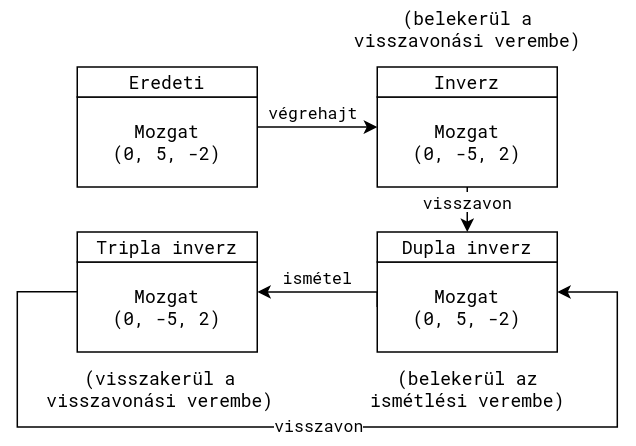
\includegraphics[width=0.5\textwidth]{parts/developer-documentation/editor/images/actions.png}
      \caption{A művelet alapú szerkesztés folyamatábrája}
\end{figure}

\subsection{Külső erőforrások kezelése}

A tervezési fázisban hamar kiderült, hogy sok időt és energiát kell fektetnünk a szerkesztő által
használt külső erőforrások tárolásának és létrehozásának módjának meghatározásába. Arra jutottunk,
hogy ezen célok teljesítéséhez saját fájlformátumokat fogunk kifejleszteni. A fejlesztés során
felmerülő igények kielégítésére végül három új fájlformátum született meg: .ascn, .amdl, és .agzm.
Mindhárom fájlformátum bináris kódolású, előállításukat és beolvasásukat a
bincode\footnote{https://github.com/bincode-org/bincode}
könyvtár végzi. Az adatokat mindegyik formátum egymásba ágyazott struktúrákban tárolja.

\pagebreak

\subsubsection{Jelenetfájl (.ascn)}

Az első általunk fejlesztett fájlformátum, a .ascn arra szolgál, hogy a szerkesztőben készített
3D jeleneteket tárolja. Az egész adatszerkezet egyetlen \emph{Scene} nevű struktúrában helyezkedik
el. Ennek a struktúrának két eleme van: \emph{camera} és \emph{world}. A \emph{Camera} struktúrában
a kamera pozíciója és forgása tárolódik, míg a \emph{World} struktúra kicsit bonyolultabb. Szintén
két eleme van: \emph{solids} és \emph{props}. Mindkét elem vektoros adatszerkezet, azaz
határozatlan mennyiségű homogén adatot tárol.

A \emph{solids} elem \emph{Solid} típusú struktúrákat tárol. Egy \emph{Solid} példány egy primitív
szilárd alakzatot modellez. Tartalmazza az alakzat csúcsait és lapjait, emellett a lapok textúráit.

A \emph{props} elem \emph{Prop} típusú struktúrákat tárol. Egy \emph{Prop} példány egy díszítőelem
adatait tárolja. Egy díszítőelemnek modell ID-je, pozíciója és forgása van.

\begin{figure}[h]
      \centering
      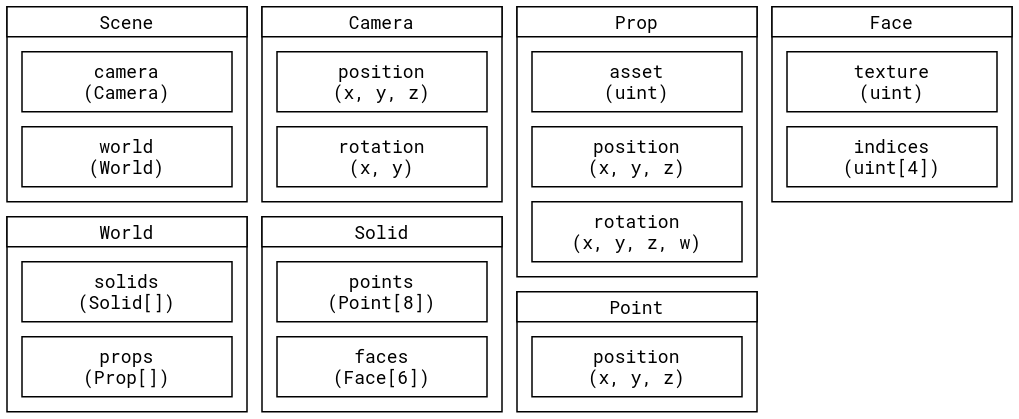
\includegraphics[width=0.8\textwidth]{parts/developer-documentation/editor/images/ascn.png}
      \caption{A .ascn fájlformátum adatszerkezetei}
\end{figure}

\pagebreak

\subsubsection{Modellfájl (.amdl)}

A .amdl fájlformátum egy tetszőlegesen komplex 3D modell tárolására szolgál, néhány korlátozással.
A formátum például nem képes animációkat kódolni, hiszen a szerkesztő nem támogatja a mozgó tárgyak
megjelenítését. A modellfájl gyökérstruktúrája \emph{Prop} névre hallgat. Két eleme van:
\emph{bounds} és \emph{meshes}. A \emph{bounds} elem a modell köré írható,
tengelyekhez igazított téglatestet tárolja. A \emph{meshes} elem vektoros adatszerkezet, ami a
modellt felépítő, textúrázott almodelleket tárolja.

\begin{figure}[h]
      \centering
      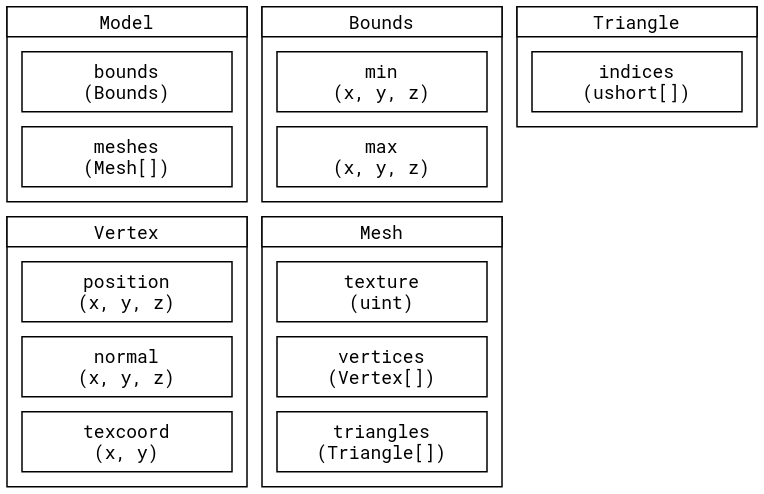
\includegraphics[width=0.6\textwidth]{parts/developer-documentation/editor/images/amdl.png}
      \caption{A .amdl fájlformátum adatszerkezetei}
\end{figure}

\subsubsection{Gizmofájl (.agzm)}

Az Archytex szerkesztő forráskódjában a gizmo szónak két jelentése is van: hivatkozhat az egér
általi mozgatást elősegítő alakzatokra, de arra a speciális 3D modellre is, aminek nincsenek
almodelljei és textúrái sem. A gizmofájl az utóbbi modellek tárolására szolgál. A három saját
fájlformátum közül ez a legegyszerűbb, hisz csak egyszerű geometriát kódol: csúcsokat, és az
azokból alkotott háromszögeket.

\begin{figure}[h]
      \centering
      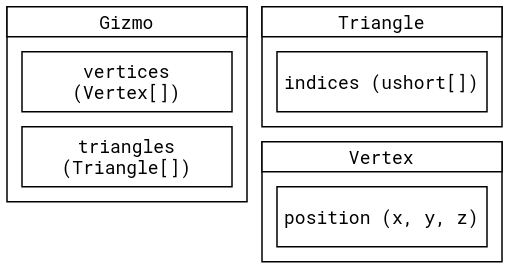
\includegraphics[width=0.4\textwidth]{parts/developer-documentation/editor/images/agzm.png}
      \caption{A .agzm fájlformátum adatszerkezetei}
\end{figure}